\documentclass{article}
\usepackage[utf8]{inputenc}

\title{EFT-DE-notes}
\author{Santiago Casas}
\date{September 2019}

\usepackage{natbib}
\usepackage{graphicx}

\begin{document}

\maketitle

\section{Introduction}
There is a theory which states that if ever anyone discovers exactly what the Universe is for and why it is here, it will instantly disappear and be replaced by something even more bizarre and inexplicable.
There is another theory which states that this has already happened.

\begin{figure}[h!]
\centering
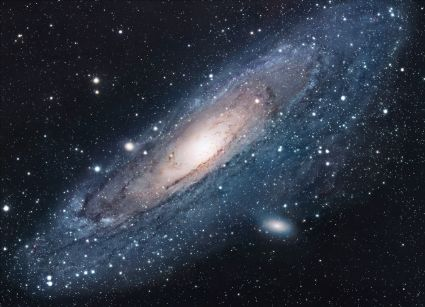
\includegraphics[scale=1.7]{universe}
\caption{The Universe}
\label{fig:universe}
\end{figure}

\section{EFT}

\subsection{Theory}

\begin{itemize}

\item The fact that we need to invoke twice an accelerated expansion phase, to explain observations, makes us wonder if fundamentally the description of GR at very large scales is correct \citep{Frusciante2019a}.

\item Expansion breaks time-translation invariance and Lorentz invariance. 

\item  Lovelock's theorem and a construction of GR from a massless spin-2 particle, prove that any modification of GR + $\Lambda$ must involve new degrees of freedom.

\item  A scalar field appears naturally as the Goldstone field of a spontaneous time symmetry breaking.  The gradient of the scalar field is time-like in unitary gauge. The fluctuations of the field disappear and become part of the metric DoFs.

\item EFT contains all possible operators compatible with those symmetries.
\item EFT contains Horndeski if second-order EOMs are imposed.
\item EFT contains also GLPV theories and DHOST.


\item  The alpha parametrization re-shuffles those operators to turn them into more physically meaningful functions.

 
\end{itemize}




\section{Conclusion}
``I always thought something was fundamentally wrong with the universe'' \citep{adams1995hitchhiker}



\bibliographystyle{plain}
\bibliography{references,EFT-DE}
%\bibliography{EFT-DE.bib}
\end{document}
